\documentclass[10pt]{article}
\usepackage[utf8]{inputenc}
\usepackage[T1]{fontenc}
\usepackage{lmodern}
\usepackage{listings}
\usepackage{makeidx}
\usepackage[toc, page]{appendix}
\usepackage{float}
\usepackage{lscape}
\usepackage{csquotes}
\usepackage{soul}
\usepackage{textcomp}
\usepackage{gensymb}
\usepackage{pdfpages}
\usepackage{caption}
\usepackage{subcaption}
\usepackage{url}
\lstset{
	keywords={SELECT, WHERE, COLUMNS, ROWS, ON, MEMBER, WITH, FROM, ALL, CROSSJOIN, TOPCOUNT, ASC, DESC, AS, PARENT, CURRENTMEMBER, CHILDREN, PREVMEMBER, NEXTMEMBER, ORDER, RANK, GENERATE},
	keywordstyle=\color{red}\bfseries
}
% \usepackage{geometry}
\usepackage[left=20mm, right=20mm, top=25mm, bottom=25mm]{geometry}
\usepackage{rotating}
\usepackage[section]{placeins}
\usepackage{chngcntr,array}
\usepackage{graphicx}
\usepackage{lscape}
\usepackage{dirtree}
\usepackage[
	breaklinks=true,
	colorlinks=true,
	linkcolor=blue,
	urlcolor=blue,
	citecolor=blue,
	bookmarks=true,
	bookmarksopenlevel=2
]{hyperref}
\usepackage{xcolor}
\usepackage{algorithm}
\usepackage{algpseudocode}
\usepackage{amsmath}
\usepackage{amsfonts}
\usepackage{amssymb}

\title{
	Machine Learning
	\\-\\
	Supervised Learning
}
\author{
	\href{mailto:brandon.alves@gatech.edu}{Brandon Alves}
}
\date{\today}

\begin{document}
	\maketitle
	\thispagestyle{empty}
	\tableofcontents
	\listoffigures
	\clearpage
	\setcounter{page}{1}
	\section{Introduction}
		\paragraph*{}
			In this article, I will present the results of various Supervised Learning methods applied on two classification problems. Those methods are:
			\begin{itemize}
				\item Decision Trees with some form of pruning;
				\item Neural Networks;
				\item Boosting;
				\item Support Vector Machines;
				\item K-Nearest Neighbors.
			\end{itemize}
			For each of them, I will discuss the results obtained, the pros and cons of using them, and the parameters that were used. I will also discuss the results when applying the methods on the two different datasets. At the end I will also compare the methods between them and highlight the best one for each dataset.

			I will present many plots on this report to show the evolution of the accuracy depending on some parameters. Those plots will be presented in the following way : the hard line represents the median precision value for a given parameter value while the tint area goes from the minimum to the maximum precision value for the given parameter value.

			The experiments on this report were performed on a computer with the following specifications:
			\begin{itemize}
				\item CPU : Intel(R) Core(TM) i7-9750H CPU @ 2.60GHz, 6 cores, 12 threads
				\item RAM : 16GB DDR4
				\item GPU : NVIDIA Quadro P620
			\end{itemize}
	\section{Datasets}
		\paragraph*{}
			In this article, I will learn over two datasets:
			\begin{itemize}
				\item \href{https://www.kaggle.com/datasets/elakiricoder/gender-classification-dataset}{Gender Classification};
				\item \href{https://www.kaggle.com/code/sngkadam/credit-card-fraud-detection/data}{Credit Card Fraud Detection}.
			\end{itemize}
		\subsection*{Gender Classification}
			\paragraph*{}
				This dataset describes some appearence characteritics. It contains 7 features and one output. The features are: long hair, width of the forehead, height of the forehead, wide nose, long nose, thin lips and the distance between nose and lips. The output feature is gender and takes value 1 for male and 0 for female. That dataset is not the most complicated. I thought it would be a good idea to start with a simple dataset to get a better understanding of the methods. It is also a good idea to start with a dataset that is not too big to avoid long training times.
		\subsection*{Credit-Card Fraud Detection}
			\paragraph*{}
				This dataset is a credit card fraud detection dataset. The dataset contains transactions made by credit cards in September 2013 by European cardholders. This dataset presents transactions that occurred in two days, where we have 492 frauds out of 284,807 transactions. The dataset is highly unbalanced, the positive class (frauds) account for 0.172\% of all transactions. It contains only numerical input variables which are the result of a PCA transformation. The only features which have not been transformed with PCA are \textit{Time} and \textit{Amount}. Feature \textit{Time} contains the seconds elapsed between each transaction and the first transaction in the dataset. The feature \textit{Amount} is the transaction amount. Feature \textit{Class} is the response variable and it takes value 1 in case of fraud and 0 otherwise.
		\subsection*{Normalisation}
			\paragraph*{}
				Some methods require the data to be scaled between 0 and 1. It also permits computation to be faster. Both the training and the testing datasets are scaled between 0 and 1. The scaling is done by dividing each value by the maximum value of the dataset. The scaling is done on the training dataset and then applied on the testing dataset.
	\section{Decision Trees}
		\paragraph*{}
			In that section I will present the results obtained when using Decision Trees with pruning. We will here discuss the influence of different parameters :
			\begin{itemize}
				\item The maximum depth of the tree;
				\item The minimum number of samples required to split an internal node;
				\item The size of the training set.
			\end{itemize}
		\paragraph*{}
			\begin{figure}[h]
				\centering
				\begin{subfigure}[]{0.45\columnwidth}
					\centering
					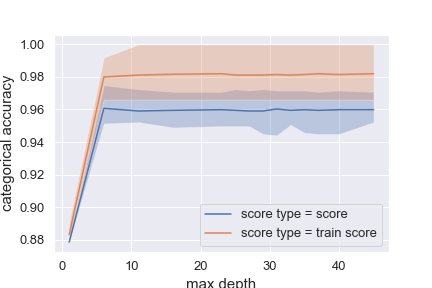
\includegraphics[width=\linewidth]{../graphics/tree_gender_max_depth_score_type_score_type.png}
					\caption{Accuracy for train and test Gender datasets}
					\label{tree:gender_train_vs_test}
				\end{subfigure}
				~
				\begin{subfigure}[]{0.45\columnwidth}
					\centering
					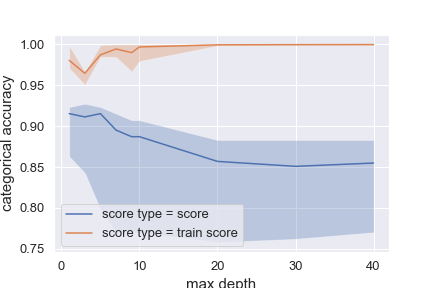
\includegraphics[width=\linewidth]{../graphics/tree_creditcard_max_depth_score_type_score_type.png}
					\caption{Accuracy for train and test Credit-Card datasets}
					\label{tree:creditcard_train_vs_test}
				\end{subfigure}
				\caption{Evolution of the Decision Tree Classifier accuracy according to the Maximum Depth of the Tree}
				\label{tree:train_vs_test}
			\end{figure}

			We begin by finding the limit of our classifier. That limit can be of two natures : overfiting or a flat level on both training and test accuracy. Figure \ref{tree:train_vs_test} represents those limits. On figure \ref{tree:creditcard_train_vs_test}, we can see that the Decision Tree method quickly overfits. Indeed the training accuracy quickly rise above 99\% while the test accuracy decreases to reach around 0.87\%. We can notice that the best score is obtained for a maximum depth value of 5. Also the score considerably decreases for a maximum depth value of bigger than 5. therefore we can conclude that only 5 out of the 28 dimensions of the input space is relevant for the classification output.

			On figure \ref{tree:gender_train_vs_test}, we can notice that the classifier does not overfit. It is interesting to constat that the score for the testing dataset happens to be better than the score for the training dataset. This is probably due to the fact that the dataset is not too big. We can also notice that the best score is obtained for a maximum depth value of 7 which means that all the dimensions of the input space are relevant for the classification output.
		\paragraph*{}
			\begin{figure}[h]
				\centering
				\begin{subfigure}[]{0.45\columnwidth}
					\centering
					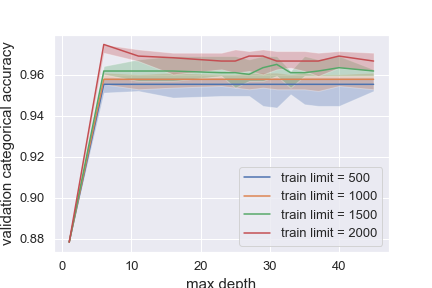
\includegraphics[width=\linewidth]{../graphics/tree_gender_max_depth_score_type_train_limit.png}
					\caption{Accuracy for train and test Gender datasets}
					\label{tree:gender_train_size_score_type_score_type}
				\end{subfigure}
				~
				\begin{subfigure}[]{0.45\columnwidth}
					\centering
					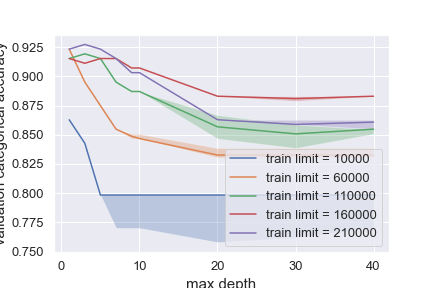
\includegraphics[width=\linewidth]{../graphics/tree_creditcard_max_depth_score_type_train_limit.png}
					\caption{Accuracy for train and test Credit-Card datasets}
					\label{tree:creditcard_train_size_score_type_score_type}
				\end{subfigure}
				\caption{Evolution of the Decision Tree Classifier accuracy according to the Size of the Training Tet}
				\label{tree:train_size_score_type_score_type}
			\end{figure}

			Let's discuss now the influence of the size of the training set on the accuracy of the classifier. Figure \ref{tree:train_size_score_type_score_type} represents the accuracy of the classifier according to the size of the training set for both datasets. As expected the accuracy of the classifier increases when the size of the training set increases. The accuracy of the classifier is also impacted by the maximum depth of the tree. Indeed, the score for all the different sizes of the training set is almost the same when the maximum depth is around 1, whereas the score differs a lot when the maximum depth of the tree increases. We can also notice that the training set with 160 000 samples gives better results than the trainingset with 210 000 samples in figure \ref{tree:creditcard_train_size_score_type_score_type}. This is probably due to the fact that the training set with 160 000 samples is more balanced than the training set with 210 000 samples, meaning that when adding those 50 000 samples, we probably introduce some noise in the training set.

			On the Gender dataset, we can see on figure \ref{tree:gender_train_size_score_type_score_type} that the accuracy of the classifier is also impacted by the size of the training set. The best score of the classifier is for a training set of 2 000 samples. We can also notice that the score is almost the same for a maximum depth between 1 and 5. This means that the training set size as more inpact on the classifier when the maximum depth of the tree is high.
		\paragraph*{}
			\begin{figure}[h]
				\centering
				\begin{subfigure}[]{0.45\columnwidth}
					\centering
					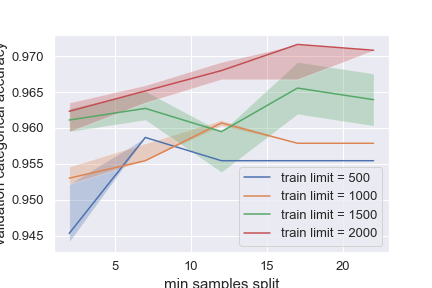
\includegraphics[width=\linewidth]{../graphics/tree_gender_min_samples_split_score_type_train_limit.png}
					\caption{Accuracy for train and test Gender datasets}
					\label{tree:tree_gender_min_samples_split_score_type_train_limit}
				\end{subfigure}
				~
				\begin{subfigure}[]{0.45\columnwidth}
					\centering
					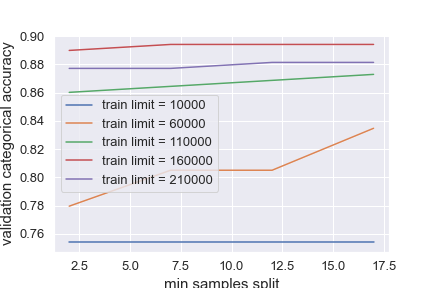
\includegraphics[width=\linewidth]{../graphics/tree_creditcard_min_samples_split_score_type_train_limit.png}
					\caption{Accuracy for train and test Credit-Card datasets}
					\label{tree:tree_creditcard_min_samples_split_score_type_train_limit}
				\end{subfigure}
				\caption{Evolution of the Decision Tree Classifier accuracy according to Minimum Number of Samples required to Split a Node}
				\label{tree:min_samples_split_score_type_score_type}
			\end{figure}

			The last parameter I will discuss is the minimum number of samples required to split an internal node. That variation is displayed on figure \ref{tree:min_samples_split_score_type_score_type}.
			In the Gender dataset, we see that this parameter has some influence. First of all we can see that this parameter lead to overfiting. In the case of the training set composed of 2 000 samples, the classifier overfits for a minimum sample split bigger than 17. But it also improve the results for all the training set sizes, when the minimum sample split is not too high.

			In the case of the Credit-Card dataset, we can see that the accuracy of the classifier is not really impacted by the minimum number of samples required to split an internal node except for the smaller datatset. Which have sense. Indeed, the smaller the dataset is the one with the biggest chance of improvment.
		\paragraph*{}
			Decision Tree is the faster method compared with all the other ones. To get those results and generate the data associated with, it took around 10 minutes.

			The decision tree classifier performs pretty well as seen above. But that method does not perform very well on highly dimensional datasets. To resolve that problem, Random Forrest can be used. Random Forrest is a method that uses multiple decision trees to classify the data. The method is based on the idea that a large number of relatively uncorrelated classifiers (trees) operating as a committee will outperform any of the individual classifiers. That method is also known as bagging.
	\section{Neural Networks}
		\paragraph*{}
			Neural Network model is the most complicated in terms of parameters in comparison with the other models. We will discuss the influence of the followings:
			\begin{itemize}
				\item The number of epochs;
				\item The use of batch normalization;
				\item The number of layers and the number of neurons per layer;
				\item The activation function;
				\item The size of the training set.
			\end{itemize}
		\paragraph*{}
			\begin{figure}[h]
				\centering
				\begin{subfigure}[]{0.45\columnwidth}
					\centering
					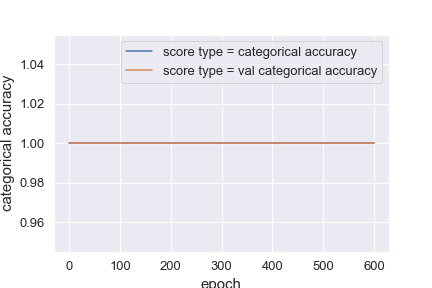
\includegraphics[width=\linewidth]{../graphics/per_gender_epoch_score_type_score_type_full.png}
					\caption{Accuracy for the train and test Gender dataset}
					\label{nn:g_train_vs_test}
				\end{subfigure}
				~
				\begin{subfigure}[]{0.45\columnwidth}
					\centering
					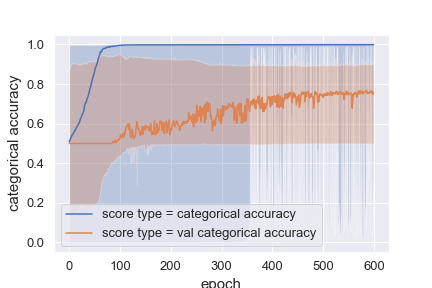
\includegraphics[width=\linewidth]{../graphics/per_creditcard_epoch_score_type_score_type_full.png}
					\caption{Accuracy for the train and test Credit-Card dataset}
					\label{nn:cc_train_vs_test}
				\end{subfigure}
				\caption{Evolution of the Neural Network Classifier accuracy according to the Number of Epochs}
				\label{nn:train_vs_test}
			\end{figure}

			The Neural Network classifier has a perfect scores on the Gender dataset. That dataset is very easy to learn over. The results are more interesting on the Credit-Card dataset. We can see on figure \ref{nn:cc_train_vs_test} that the score of the classifier goes up with the number of epochs which seems totally fair. We notice that the classifier does not overfit the training set.
		\paragraph*{}
			\begin{figure}[h]
				\centering
				\begin{subfigure}[]{0.45\columnwidth}
					\centering
					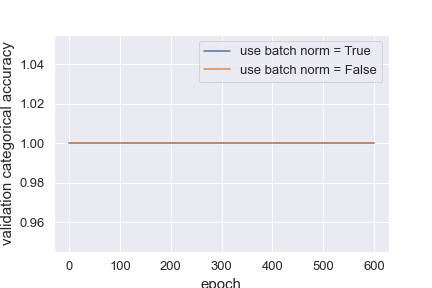
\includegraphics[width=\linewidth]{../graphics/per_gender_epoch_score_type_use_batch_norm.png}
					\caption{Accuracy with and without batch normalization for Gender dataset}
					\label{nn:g_bn}
				\end{subfigure}
				~
				\begin{subfigure}[]{0.45\columnwidth}
					\centering
					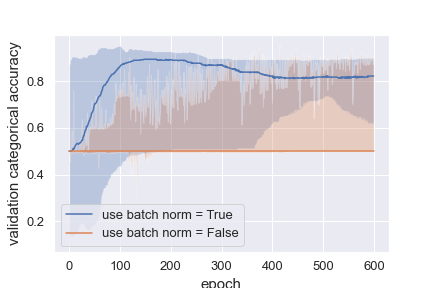
\includegraphics[width=\linewidth]{../graphics/per_creditcard_epoch_score_type_use_batch_norm.png}
					\caption{Accuracy with and without batch normalization for Credit-Card dataset}
					\label{nn:cc_bn}
				\end{subfigure}
				\caption{Evolution of the Neural Network Classifier accuracy according to the use of Batch Normalization}
				\label{nn:bn}
			\end{figure}

			The parameter that affects the most the accuracy of the calssifier is the use of a batch normalization as we can see on figure \ref{nn:bn}. We know that the use of a batch normalization permits to decrease the number of training epochs required to train a neural network. We can see on figure \ref{nn:cc_bn} that not using batch normalisation does not even permit to reach a score of 0.5. The use of batch normalization is mandatory to get a good score on the Credit-Card dataset.
		\paragraph*{}
			\begin{figure}[h]
				\centering
				\begin{subfigure}[]{0.45\columnwidth}
					\centering
					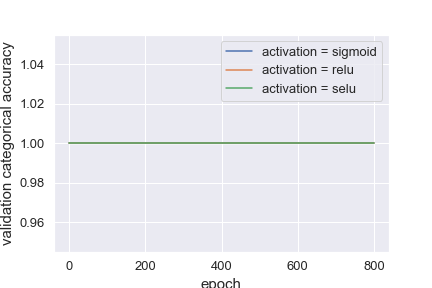
\includegraphics[width=\linewidth]{../graphics/per_gender_epoch_score_type_activation.png}
					\caption{Accuracy for different activation functions on Gender dataset}
					\label{nn:g_act}
				\end{subfigure}
				~
				\begin{subfigure}[]{0.45\columnwidth}
					\centering
					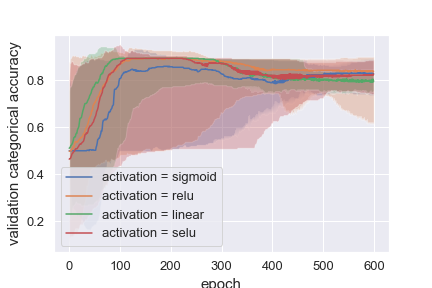
\includegraphics[width=\linewidth]{../graphics/per_creditcard_epoch_score_type_activation.png}
					\caption{Accuracy for different activation functions on Credit-Card dataset}
					\label{nn:cc_act}
				\end{subfigure}
				\caption{Evolution of the Neural Network Classifier accuracy according to the Activation Function}
				\label{nn:activation}
			\end{figure}

			Let's discuss the impact of the activation function. The impact of the activation function is not as important as the batch normalization. We can see on figure \ref{nn:activation} that the accuracy is not very different between the different activation functions. On the Credit-Card dataset, on figure \ref{nn:cc_act}, the activation function that gets the worse results is the \textit{sigmoid}.
		\paragraph*{}
			\begin{figure}[h]
				\centering
				\begin{subfigure}[]{0.45\columnwidth}
					\centering
					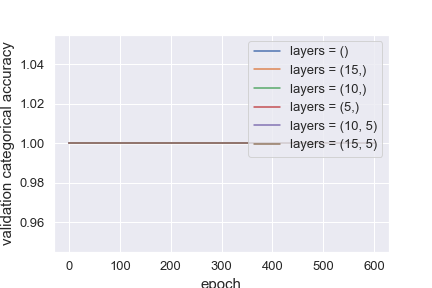
\includegraphics[width=\linewidth]{../graphics/per_gender_epoch_score_type_layers.png}
					\caption{Accuracy for different layers on Gender dataset}
					\label{nn:g_layers}
				\end{subfigure}
				~
				\begin{subfigure}[]{0.45\columnwidth}
					\centering
					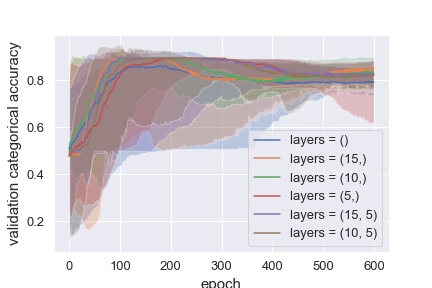
\includegraphics[width=\linewidth]{../graphics/per_creditcard_epoch_score_type_layers.png}
					\caption{Accuracy for different layers on Credit-Card dataset}
					\label{nn:cc_layers}
				\end{subfigure}
				\caption{Evolution of the Neural Network Classifier accuracy according to the Number of Layers}
				\label{nn:layers}
			\end{figure}

			Another parameter that affected the score of the classifier is the number of layers and the number of nodes they contains. We can see on figure \ref{nn:layers} that the accuracy depends on the layers. For the Gender dataset, results are the same for both layers we trained our network with. In fact not using layers (output directly connected to input) still gives a 100\% fit as we can see on figure \ref{nn:g_layers}.

			On figure \ref{nn:cc_layers} we can see that the choose of layers does not have a big impact on the accuracy. The best results are obtained with 2 layers. The number of nodes in the layers does not have a big impact on the accuracy. The best results are obtained with 10 nodes in the first layer and 5 nodes in the second layer. But the results are not very different with only one layer with 5 nodes in it.
		\paragraph*{}
			\begin{figure}[h]
				\centering
				\begin{subfigure}[]{0.45\columnwidth}
					\centering
					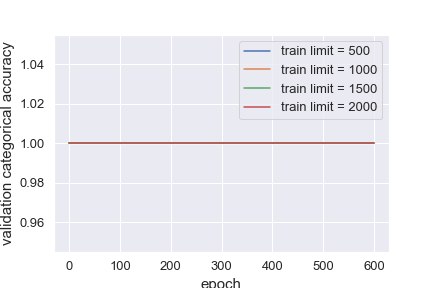
\includegraphics[width=\linewidth]{../graphics/per_gender_epoch_score_type_train_limit.png}
					\caption{Accuracy for different training dataset sizes on Gender dataset}
					\label{nn:g_tl}
				\end{subfigure}
				~
				\begin{subfigure}[]{0.45\columnwidth}
					\centering
					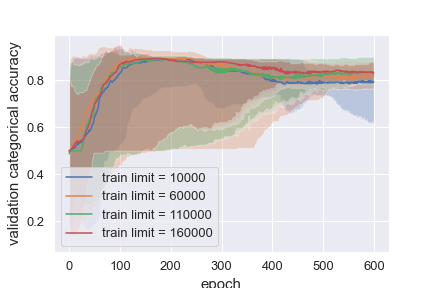
\includegraphics[width=\linewidth]{../graphics/per_creditcard_epoch_score_type_train_limit.png}
					\caption{Accuracy for different training dataset sizes on Credit-Card dataset}
					\label{nn:cc_tl}
				\end{subfigure}
				\caption{Evolution of the Neural Network Classifier accuracy according to the Training Dataset Size}
				\label{nn:size}
			\end{figure}

			One interesting thing in that case is that the training size does not seem to have a big impact on the classification score. We can see on figure \ref{nn:cc_tl} that the accuracy is not very different between the different training sizes. For example we have pretty much the same accuracy for a 1 000 and a 160 000 training size.
		\paragraph*{}
			In terms of computation time, our Neural Network classifier is the third slowest. In addition, the memory used in the learning process was also very high. It took 3h30m to train the neural network on both datasets.

			I saw that, on the Credit-Card dataset, it is not easy to find a good tuning for the neural network for all these parameters to obtain good results.
	\section{Boosting}
		\paragraph*{}
			Let's now discuss the influence of the followings parameters on the accuracy of the Boosting classifier:
			\begin{itemize}
				\item The number of boosting stages to perform;
				\item The maximum depth of an individual regression estimator;
				\item The minimum number of sample needed to split a node of an estimator;
				\item The size of the training set.
			\end{itemize}
		\paragraph*{}
			\begin{figure}[h]
				\centering
				\begin{subfigure}[]{0.45\columnwidth}
					\centering
					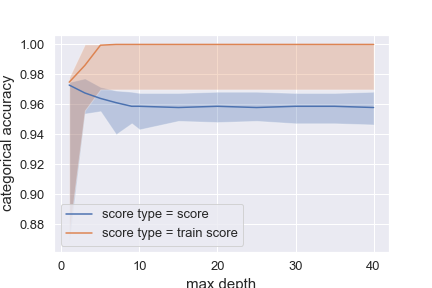
\includegraphics[width=\linewidth]{../graphics/boost_gender_max_depth_score_type_score_type.png}
					\caption{Accuracy for the train and test Gender dataset}
					\label{boost:g_train_vs_test}
				\end{subfigure}
				~
				\begin{subfigure}[]{0.45\columnwidth}
					\centering
					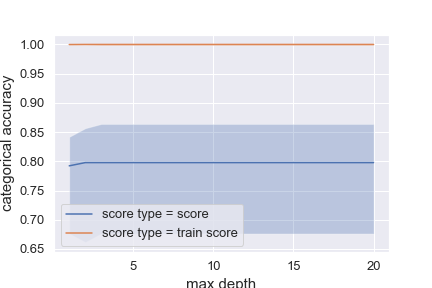
\includegraphics[width=\linewidth]{../graphics/boost_creditcard_max_depth_score_type_score_type.png}
					\caption{Accuracy for the train and test Credit-Card dataset}
					\label{boost:cc_train_vs_test}
				\end{subfigure}
				\caption{Evolution of the Boosting Classifier accuracy according to the Maximum Depth of an Estimator}
				\label{boost:train_vs_test}
			\end{figure}

			First, we can see that the accuracy of the Boosting classifier is very good on the Gender dataset and pretty good on the Credit-Card dataset.
			On figure \ref{boost:train_vs_test}, we can see the accuracy of both classifier according to the maximum depth of an individual regression estimator. For the Gender dataset, it is interesting to notice that the score of the classifier is the best when the maximum depth is 1. That means that each tree of the Boosting classifier is a simple node. The Gender dataset is probably too simple to benefits from higher maximum depth values.

			For the Credit-Card dataset, the accuracy is the best when the maximum depth is higher to 2. We also notice that the classifier does not overfit. Unlike in the case of the Gender dataset, the Credit-Card dataset benefits from higher maximum depth values.
		\paragraph*{}
			\begin{figure}[h]
				\centering
				\begin{subfigure}[]{0.45\columnwidth}
					\centering
					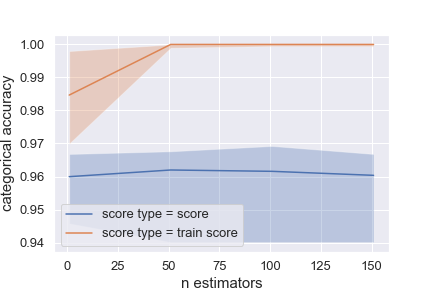
\includegraphics[width=\linewidth]{../graphics/boost_gender_n_estimators_score_type_score_type.png}
					\caption{Accuracy for the train and test Gender dataset, for $maxdepth=1$}
					\label{boost:g_train_vs_test_es}
				\end{subfigure}
				~
				\begin{subfigure}[]{0.45\columnwidth}
					\centering
					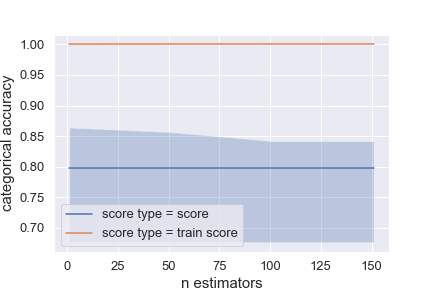
\includegraphics[width=\linewidth]{../graphics/boost_creditcard_n_estimators_score_type_score_type.png}
					\caption{Accuracy for the train and test Credit-Card dataset, for $maxdepth=3$}
					\label{boost:cc_train_vs_test_es}
				\end{subfigure}
				\caption{Evolution of the Boosting Classifier accuracy according to the Number of Estimator used for a given maximum depth}
				\label{boost:train_vs_test_es}
			\end{figure}

			Let's now discuss the impluence of the number of estimators. Results are presented on figure \ref{boost:train_vs_test_es}.
			In the case of the Gender dataset, we can see that the accuracy is the higher for a number of estimators bigger than 50. This is interesting because we saw that the best fit for the Gender dataset was trees with only one node. So, it seems that the Boosting classifier is able to combine a lot of simple trees to obtain a good accuracy.

			For the Credit-Card dataset, presented on figure \ref{boost:cc_train_vs_test_es}, we can see that the score is not dependent on the number of estimators, which means that a single Decision Tree was enough to obtain a good accuracy.
		\paragraph*{}
			\begin{figure}[h]
				\centering
				\begin{subfigure}[]{0.45\columnwidth}
					\centering
					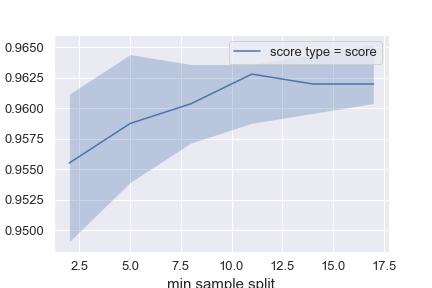
\includegraphics[width=\linewidth]{../graphics/boost_gender_min_sample_split_score_type_score_type.png}
					\caption{Accuracy for the train and test Gender dataset, for $trainlimit=2000$ and $maxdepth\ge1$}
					\label{boost:g_train_vs_test_ms}
				\end{subfigure}
				~
				\begin{subfigure}[]{0.45\columnwidth}
					\centering
					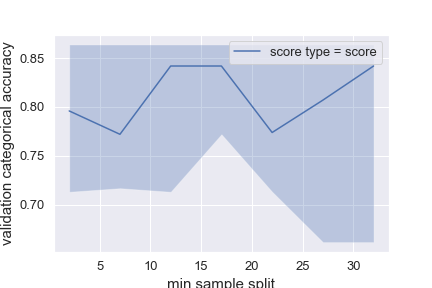
\includegraphics[width=\linewidth]{../graphics/boost_creditcard_min_sample_split_score_type_score_type.png}
					\caption{Accuracy for the train and test Credit-Card dataset, for $trainlimit=11000$ and $maxdepth\geq1$}
					\label{boost:cc_train_vs_test_ms}
				\end{subfigure}
				\caption{Evolution of the Boosting Classifier accuracy according to the Minimum Number of Sample to Split an Estimator's node for a given size of training and maximum depth}
				\label{boost:train_vs_test_ms}
			\end{figure}

			I present on figure \ref{boost:train_vs_test_ms} the influence of the parameter that set the minimum number of samples required to split an internal node.
			In the figure \ref{boost:g_train_vs_test_ms}, we can see that for the Gender dataset, thhat parameter increases a little bit the score of the classifier. But because we saw the perfect fit of the classifier with a maximum depth of 1, we wouldn't really care about that value.

			For the Credit-Card dataset, presented on figure \ref{boost:cc_train_vs_test_ms}, we can see that the best score is for a value between 12 and 17. It is interesting. The fact is I was not able to train as much data I would have liked for this dataset, because of computation time. Perhaps, with more data, result would have been more understanding.

		\paragraph*{}
			\begin{figure}[h]
				\centering
				\begin{subfigure}[]{0.45\columnwidth}
					\centering
					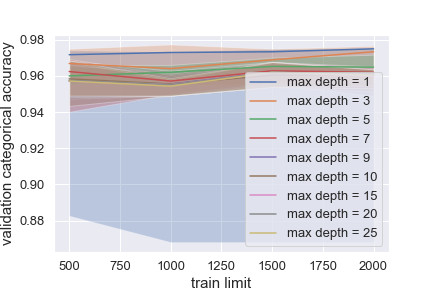
\includegraphics[width=\linewidth]{../graphics/boost_gender_train_limit_score_type_max_depth.png}
					\caption{Accuracy for the train and test Gender dataset, for different train max depth values}
					\label{boost:g_train_limit}
				\end{subfigure}
				~
				\begin{subfigure}[]{0.45\columnwidth}
					\centering
					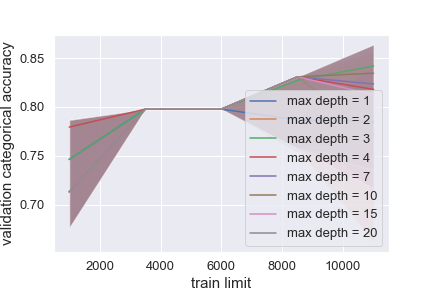
\includegraphics[width=\linewidth]{../graphics/boost_creditcard_train_limit_score_type_max_depth.png}
					\caption{Accuracy for the train and test Credit-Card dataset, for different train max depth values}
					\label{boost:cc_train_limit}
				\end{subfigure}
				\caption{Evolution of the Boosting Classifier accuracy according to the Training Set Size}
				\label{boost:train_limit}
			\end{figure}

			In figure \ref{boost:train_limit}, I present the accuracy of the classifier according to the training set size.
			In the Gender dataset, we can see that the accuracy does not change a lot when the training set size is increased. That could mean the that the data is nnot very complex and well balanced.

			In the Credit-Card dataset, presented on figure \ref{boost:cc_train_limit}, as expected, we can see that the accuracy increases when the training set size increases. There is that weird flat for a training set size between 3 500 and 6 000 were independent of the maximum depth, the score is the same. I could not explain why.
			I was not able to train more data due to the time computation of the Boosting classifier.

		\paragraph*{}
			In terms of computation time, the Boosting Classifier is the slowest of all the classifiers I trained. To get the results and generate the data, it around 1h10m.

			To conclude, we saw that Boosting classifier gets pretty good results. It seems to not tend to overfitting, which is a good thing. But it is the slowest of all the classifiers I trained. So, it would not really be a good choice for a real time application. For the Gender dataset, we saw that a Decision Tree was enough. For the Credit-Card dataset, I cannot really compare because I didn't trained it with enough data.
	\section{Support Vector Machines}
		\paragraph*{}
			In this section we will discuss about the Support Vector Machines classifier. We will see the influence of the followings parameters:
			\begin{itemize}
				\item The penalty of the error term (C value);
				\item The kernel function;
				\item The training set size.
			\end{itemize}

		\paragraph*{}
			\begin{figure}[h]
				\centering
				\begin{subfigure}[]{0.45\columnwidth}
					\centering
					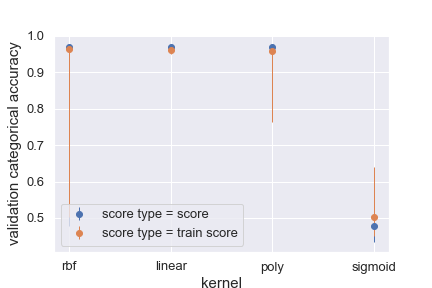
\includegraphics[width=\linewidth]{../graphics/svm_gender_kernel_score_type_score_type.png}
					\caption{Accuracy for the train and test Gender datasets}
					\label{svm:g_train_vs_test}
				\end{subfigure}
				~
				\begin{subfigure}[]{0.45\columnwidth}
					\centering
					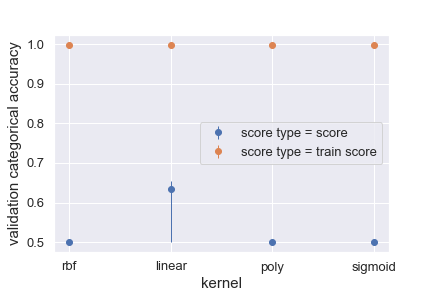
\includegraphics[width=\linewidth]{../graphics/svm_creditcard_kernel_score_type_score_type.png}
					\caption{Accuracy for the train and test Credit-Card datasets}
					\label{svm:cc_train_vs_test}
				\end{subfigure}
				\caption{Evolution of the SVM Classifier accuracy according to the Kernel}
				\label{svm:train_vs_test}
			\end{figure}

			The parameter that seems to have the biggest impact is the kernel choosed.
			In figure \ref{svm:train_vs_test}, we can see the impact on the score for both datasets. In the case of the Gender dataset, on figure \ref{svm:g_train_vs_test}, we see that the accuracy is pretty much the same for all the kernels except for the \textit{sigmoid} where the accuracy falls down to 0.45. The accuracy is around 0.98 for the other kernels : linear, polynomial (3rd degree) and the radial basis function. The score for the linear kernel clearly show that the data are linearly separable.

			In the case of the Credit-Card dataset, on figure \ref{svm:cc_train_vs_test}, we see that the accuracy is better for the linear kernel, with an accuracy around 0.61. The other kernels don't perform very well.

		\paragraph*{}
			\begin{figure}[h]
				\centering
				\begin{subfigure}[]{0.45\columnwidth}
					\centering
					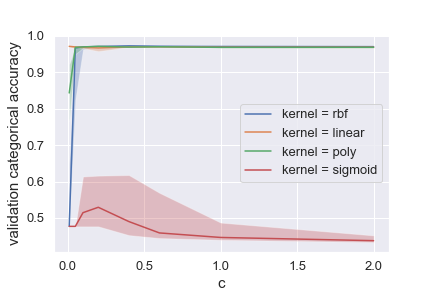
\includegraphics[width=\linewidth]{../graphics/svm_gender_c_score_type_kernel.png}
					\caption{Accuracy for test Gender dataset according to different kernels}
					\label{svm:g_c}
				\end{subfigure}
				~
				\begin{subfigure}[]{0.45\columnwidth}
					\centering
					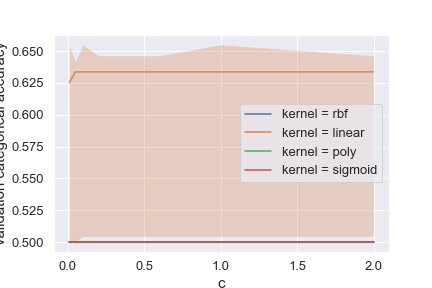
\includegraphics[width=\linewidth]{../graphics/svm_creditcard_c_score_type_kernel.png}
					\caption{Accuracy for test Credit-Card dataset according to different kernels}
					\label{svm:cc_c}
				\end{subfigure}
				\caption{Evolution of the SVM Classifier accuracy according to the C value}
				\label{svm:c}
			\end{figure}

			Let's now study the impact of the C parameter. In SVM, we are searching for a hyperplane with the largest minimum margin, and a hyperplane that correctly separates as many instances as possible. The problem is that it is not always possible to get both. The C parameter determines how great our desire is for the latter. Figure \ref{svm:c} presents the accuracy for the test dataset according to the C value.

			For Gender dataset, we can see, on figure \ref{svm:g_c} that the C value doesn't have a big impact on the accuracy. The accuracy is around 0.98 for all the C values bigger than 0.01, except for the \textit{sigmoid} kernel where the accuracy falls down tunder 0.5. Once again, because the data are linearly separable, the accuracy is pretty much the same for all the C values bigger than 0.01.
			The strength of the regularization is inversely proportional to C. So, the smaller C is, the stronger the regularization is. Having a C value to small means that we are considering the margin too much, and we are not allowing enough errors. So, we are underfitting the data.

			In the case of the Credit-Card dataset, on figure \ref{svm:cc_c}, we can see that the accuracy is neither really affected by the regularisation parameter for both kernels.
		\paragraph*{}
			\begin{figure}[h]
				\centering
				\begin{subfigure}[]{0.45\columnwidth}
					\centering
					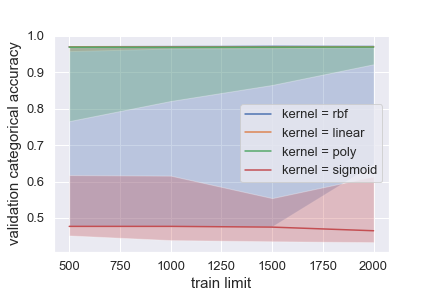
\includegraphics[width=\linewidth]{../graphics/svm_gender_train_limit_score_type_kernel.png}
					\caption{Accuracy for test Gender dataset for different kernels}
					\label{svm:g_train_limit}
				\end{subfigure}
				~
				\begin{subfigure}[]{0.45\columnwidth}
					\centering
					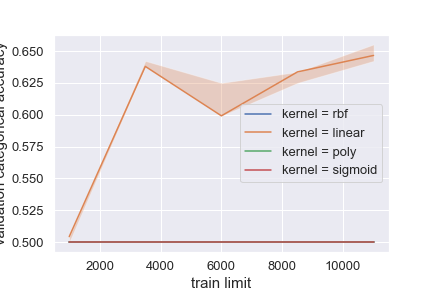
\includegraphics[width=\linewidth]{../graphics/svm_creditcard_train_limit_score_type_kernel.png}
					\caption{Accuracy for test Credit-Card dataset for different kernels}
					\label{svm:cc_train_limit}
				\end{subfigure}
				\caption{Evolution of the SVM Classifier accuracy according to the Size of the Training Set}
				\label{svm:train_limit}
			\end{figure}

			The last parameter I will discuss for SVM is the training size. The results are presented on figure \ref{svm:train_limit}.
			For the Gender dataset, we can see on figure \ref{svm:g_train_limit} that the accuracy is pretty much the same for all the training set sizes, with the working kernels. That dataset is indeed too easely separable.

			For the Credit-Card dataset, we can see on figure \ref{svm:cc_train_limit} that the accuracy for the linear kernel is impacted by the training set size. There is that hollow betwenn 4 000 and 8 000 samples which means that we probably introduced outliers in the data. But the accuracy seems overall increasing with the training set size. I was not able to train more data due to the time computation of the SVM classifier.

		\paragraph*{}
			Concerning time efficiency, the SVM classifier is one of the slowest. To get those results and generate the data associated with, it took around 25 minutes (knowing that I didn't train the SVM classifier with more than 11 000 samples for the Credit-Card dataset).

			In conlusion, SVM does not perform very well on the most difficult dataset, the Credit-Card one. I think the most important for SVM working well is the choice of the kernel function as seen above. In the overhand, data are not always linearly separable. In the case of the Credit-Card dataset, it seems that it is not the case. So SVM does not seem to be a good option.
	\section{K-Nearest Neighbors}
		\paragraph*{}
			Here I will discuss the results obtained using a K-Nearest Neighbors classifier. We will see the influence on the accuracy of the classifier of:
			\begin{itemize}
				\item The number of neighbors;
				\item The distance metric (p-norm);
				\item The size of the training set.
			\end{itemize}
			By design, the accuracy on the training set is always 100\% for KNN, so I will not display it on the plots.

		\paragraph*{}
			\begin{figure}[h]
				\centering
				\begin{subfigure}[]{0.45\columnwidth}
					\centering
					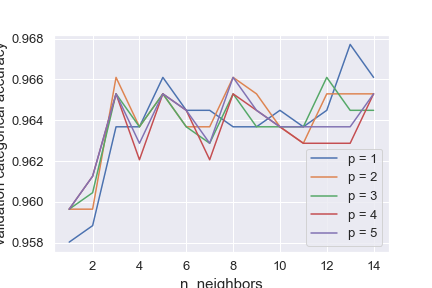
\includegraphics[width=\linewidth]{../graphics/knn_gender_neighbors.png}
					\caption{Evolution of the accuracy according to the number of neighbors on Gender dataset, with $train\_limit = 2000$}
					\label{knn:g_neighbors}
				\end{subfigure}
				~
				\begin{subfigure}[]{0.45\columnwidth}
					\centering
					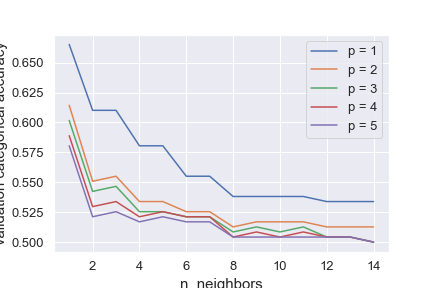
\includegraphics[width=\linewidth]{../graphics/knn_creditcard_neighbors.png}
					\caption{Evolution of accuracy according to the number of neighbors on Credit-Card dataset, with $train\_limit = 90000$}
					\label{knn:cc_neighbors}
				\end{subfigure}
				\caption{Evolution of the K-NN Classifier accuracy according to the Number of Neighbors}
				\label{knn:neighbors}
			\end{figure}

			On figure \ref{knn:neighbors}, I present the effect of those parameters on the classification score.
			For the Credit-Card dataset, we can notice on figure \ref{knn:cc_neighbors} that the norm used for the distance metric has a consequent influence on the classification accuracy. The accuracy is better when using the Manhattan norm ($p = 1$). This is not a surprise as higher norm are generally inadequate to measure distances on highly dimensional spaces. In the case of the Gender datatset, the norm used doesn't seem to have a big influence on the accuracy.

		\paragraph*{}
			On figures \ref{knn:cc_neighbors} we can see that the accuracy of the classifier is better for a small number of neighbors. K-NN is a non-parametric classifier. It is not able to generalize the data, so it is better to use a small number of neighbors. We usually increase the research perimeter to be more resilient to noise but here the data do not allow us such a liberty. This is particularly true in the Credit-Card dataset where the fraud are really close to legal transactions.

			On figure \ref{knn:g_neighbors}, we can see that the accuracy is better for a number of neighbors bigger than 3. In the case of the Gender dataset, the data are more separated and we can afford to increase the number of neighbors.
		\paragraph*{}
			\begin{figure}[h]
				\centering
				\begin{subfigure}[]{0.45\columnwidth}
					\centering
					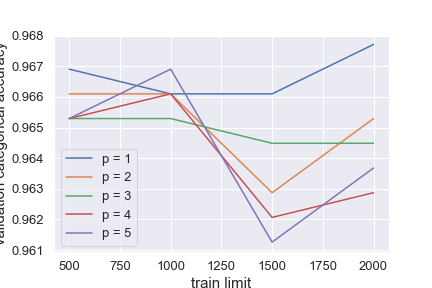
\includegraphics[width=\linewidth]{../graphics/knn_gender_train_limit.png}
					\caption{Evolution of accuracy according to the number of training examples on Gender dataset, with $n\_neighbors = 13$}
					\label{knn:g_train_limit}
				\end{subfigure}
				~
				\begin{subfigure}[]{0.45\columnwidth}
					\centering
					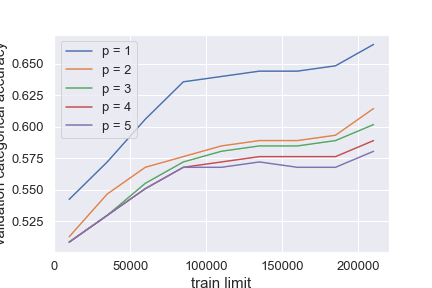
\includegraphics[width=\linewidth]{../graphics/knn_creditcard_train_limit.png}
					\caption{Evolution of accuracy according to the number of training examples on Credit-Card dataset, with $n\_neighbors = 1$}
					\label{knn:cc_train_limit}
				\end{subfigure}
				\caption{Evolution of the K-NN Classifier accuracy according to the Size of the Training Set}
				\label{knn:train_limit}
			\end{figure}

			On figure \ref{knn:train_limit}, we can see that the accuracy of the classifier is better for an important number of training examples. Also the classifier doesn't overfit. On figure \ref{knn:g_train_limit}, we can see that the accuracy decreases for a number of training examples between 1 000 and 1 500. But it keeps having a very good score. I don't really know why. The samples introduced probably where not well representative of the data.

		\paragraph*{}
			Concerning time efficiency, the K-NN classifier achieve a good performance. To get those results and generate the data associated with, it took around 25 minutes.

			In comparison with the other methods, K-NN didn't  perform well on the Credit-Card dataset. Having a discussion with an expert of the dataset would be a good idea for designing a distance metric that is better suited to the problem. Indeed, the distance metric is the key to success with K-NN. So it is important to choose the most appropriate one.
	\section{Conclusion}
		\paragraph*{}
			The best classifier for the Gender dataset was the Neural Network. The best classifier for the Credit-Card dataset was the Decision Tree. It is interesting to see that the most complex dataset got best score with one of the simpliest classifier, and the most simple dataset got best score with one of the most complex classifier in terms of parameters.

			The most complicated in machine learning is without doubt the tuning of the parameters. It is a very time consuming task. It is also a very important task. The choice of the parameters is the key to success. That is why the domain knowledge is so important.

			We also saw that the datasets are all different. The quantity of data is also fundamental in machine learning.
\end{document}
